%%Author: Andy Goetz
%%Date Modified: 10-7-09
%%License: Ask me before reproducing/modifying, etc.


\documentclass[conference]{IEEEtran}
\usepackage{tikz}
\usetikzlibrary{shapes,arrows}
\usepackage{flushend}
\usepackage{hyperref}

\newcommand{\E}{\mathrm{E}}
\newcommand{\Tran}{{\mkern-1.5mu\mathsf{T}}}
\newcommand{\Herm}{{\mathsf{H}}}


\newcommand{\centerimage}[3]{
\begin{figure}[!h]  
\centering
#1
\caption{#2}
\label{#3}
\end{figure}}

\newcommand{\doubleimage}[3]{
\begin{figure*}[!t]  
\centering
#1
\caption{#2}
\label{#3}
\end{figure*}}




%Make sure you have the file ShumanNote.scy in the same directory as
%this one. It has contains the style sheet for ECE111, and is needed
%to standardize the layout of LateX documents created for the class.
\usepackage{listings}
\usepackage{ucs}
\usepackage[utf8x]{inputenc}
%This package is used to line up pictures 
\usepackage{graphicx}
\usepackage{fancyvrb}
\usepackage{listings}
%allows cursive font
\usepackage{amssymb}
\usepackage{amsmath}



%allows hyperlinks 
%\usepackage{hyperref}

\begin{document}

%% These commands allow me to use cursive letter for things such as
%% length.  Note that on ubuntu linux, this required installation of
%% the package 'texlive-fonts-extra'. 
%% Taken from
%% http://www.latex-community.org/forum/viewtopic.php?f=5&t=1404&start=0
\newenvironment{frcseries}{\fontfamily{frc}\selectfont}{}
\newcommand{\textfrc}[1]{{\frcseries#1}}
\newcommand{\mathfrc}[1]{\text{\textfrc{#1}}}


\title{A Comparison of Image Sharpening Algorithms}
\author{Andy Goetz}

\author{\IEEEauthorblockN{Andy Goetz}
\IEEEauthorblockA{Portland State University\\
Email: agoetz@pdx.edu}}


\maketitle

\begin{abstract}
  Several different image sharpening techniques are evaluated,
  including Lanczos Interpolation, and Variable Pixel Linear
  Reconstruction. These are combined with the `Lucky Imaging'
  technique, to improve the effective resolution of planetary imaging
  problems. These techniques ended up a subjective increase in image
  sharpness, but more work needs to be done to evaluate them
  objectively.
  
\end{abstract}

\begin{IEEEkeywords}
Lucky Imaging, Variable Pixel Linear Reconstruction
\end{IEEEkeywords}

\section{Introduction}

Astronomers depend on astronomical images gathered through telescopes
in order to do their work. It follows that any increase in the
accuracy of these images enables scientists to move the field
forward. Every time a new telescope is constructed, for example the
Keck Observatory, or the Hubble Space Telescope, the field of
astronomy makes a quantum leap.

Therefore, techniques for increasing the sharpness of astronomic
images has inherent value. In this paper, several techniques for
increasing apparent image resolution are discussed.

\section{Background}

Before describing these algorithms, it is worth reviewing how the
different sources of error add in an image formed by a telescope
located on planet earth.

\centerimage{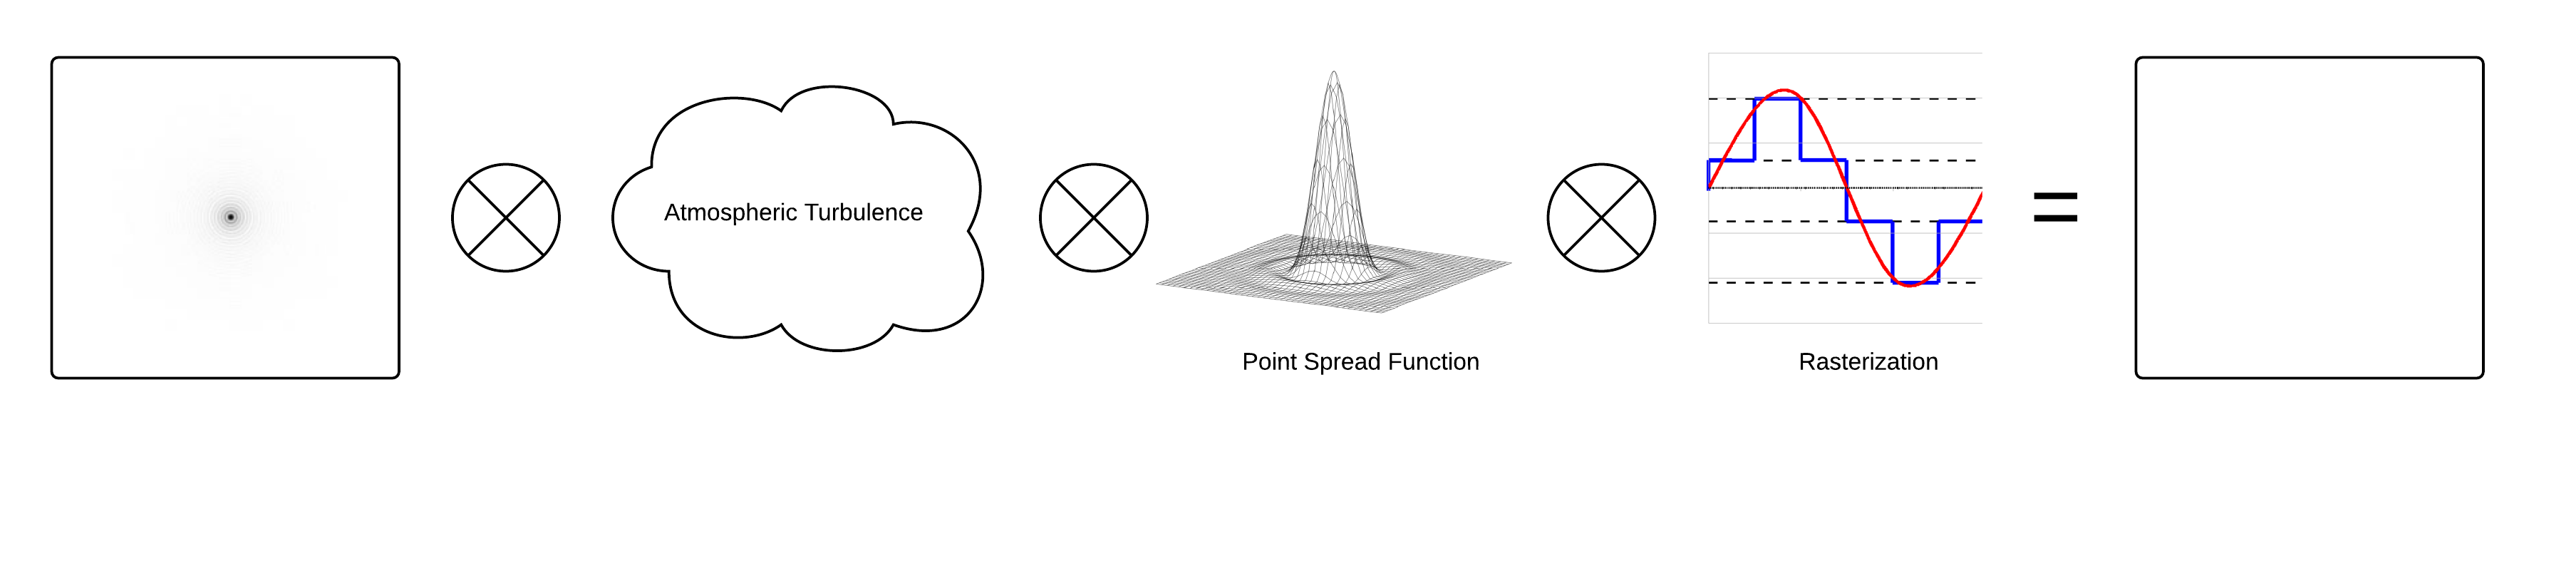
\includegraphics[width=0.9\columnwidth]{img/terrestrial_imaging.png}}{Terrestrial Imaging}{fig:imaging}

As shown in figure \ref{fig:imaging}, there are several sources of
error in the terrestrial imaging process.

\begin{itemize}
  \item Atmospheric Turbulence \\ 
  \item Point Spread Function of Optics \\
  \item Rasterization and Quantization of Imaging Device
\end{itemize}

The largest influence on the quality of terrestrial imaging is the
quality of the atmospheric seeing. Depending on temperature, the index
of refraction of air will change. This means that the transfer
function of the air with respect to the optical signal is a function
of the local turbulence of the wind. This is why earth-based
observatories tend to be located on top of mountains: This places them
above the weather patterns that can cause an increase in
turbulence.

One technique for dealing with this distortion is known as Lucky
Imaging\cite{law2007lucky}. In a nutshell, many images of the same
astronomical feature are captured, and only the sharpest images are
combined together in order to create a better image.

The quality of atmospheric seeing is usually what limits traditional
astrophotography. The size of the effective point spread function
determined from astronomical seeing conditions is known as the Full
With at Half Maximum\cite{FWHM}. The best possible seeing conditions
on the surface of the earth correspond to a FHWM of about 0.4
arcseconds.

Another source of error is the point spread function of the telescope
optics. Optical abberation can come from a variety of sources, for
example lens misalignment or coma error. 

However, even a perfect optical system is limited by the diffraction of light to
have a minimum feature size that is resolvable.

This minimum is approximated by:

\begin{equation}
  \theta = 1.22 \frac{\lambda}{D}
\end{equation}

Where $\theta$ is the angular resolution of the optical system,
$\lambda$ is the wavelength of light being imaged, and $D$ is the
diameter of the lens' aperture.

As you can see, the larger the aperture of the telescope, the smaller
a feature that can be resolved. For reference, the Hale Telescope at
the Palomar Observatory featurs a 200 inch aperture, which corresponds
to an angular resolution of green light of:

\begin{equation}
 1.22 \frac{0.5 \mathrm{ \mu{}m}}{5.1\mathrm{ m}} = 0.0005\mathrm{ arcseconds} 
\end{equation}

This is much higher than the best seeing conditions possible, which
shows the limitations of the atmosphere. 

The last main component of telescopic imaging is electronics of the
actual imaging. The optical sensor must quantize and rasterize the
light falling on it, and is limited by the size of the individual
pixels of the sensor. The imaging camera of the Hale Telescope has an
angular resolution of 0.18 arcseconds per pixel. Again, this is much
higher than the actual resolution of the telscope, and limits the
actual resolution of the telscope.

\section{Image Processing Overview}

As shown in the previous section, there are several elements combined
together that make terrestrial imaging difficult. Fortunately, for us
however, there is a way to reduce their impact:
oversampling. Oversampling involves combining multiple images of the
same target to increase the signal to noise ratio. Since most
astrophotography involves imaging phenomena that change on extremely
long timescales, we can combine multiple exposures into a single image
to increase image quality. This was the technique undertaken for this
project, with a workflow shown in figure \ref{fig:workflow}.

\centerimage{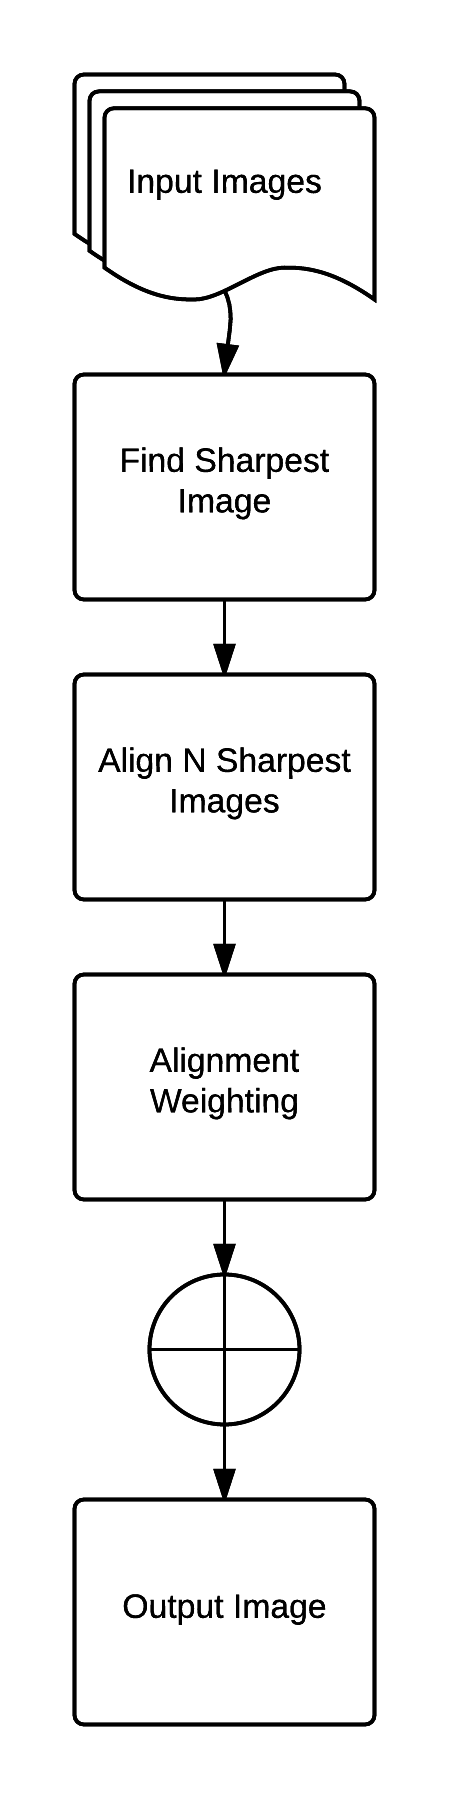
\includegraphics{img/algorithm.png}}{Image Processing Workflow}{fig:workflow}

\section{Evaluating Image Sharpness}
The first task in the imaging workflow involves determining the
sharpness of the individual exposures. When imaging point sources,
such as stars, the sharpness of the image can be evaluated using the
Strehl Ratio\cite{strehl}, which is the ratio of the peak magnitude of
the point spread function of the optics in the image compared to an
ideal optical system. This can be estimated as the highest magnitude
of a region of the image. Higher magnitude implies higher sharpness.

While appropriate for imaging point sources, the Strehl Ratio is less
useful on non-point source images, such as planets. In this case, the
Laplacian is a better representation of the sharpness of individual
regions of the image: 

\begin{equation}
  \mathbf{D}^2_{xy} =
  \begin{bmatrix}
    1 & 1 & 1 \\
    1 & -8 & 1 \\
    1 & 1 & 1
    \end{bmatrix}
\end{equation}

This is the sharpness operator chosen for this project. In addition to
being used to choose the sharpest image to use as a base for further
operations, individual regions of each image are weighted by their
local sharpness.

In order to increase the quality of the final output image, multiple
source images are combined together. The laplacian sharpness metric is
used to choose a percentage of the source images that are considered
most sharp. 

\section{Frame Alignment}
Once the source images have been selected, they must be aligned. Since
the earth rotates around the sun once every 24 hours\cite{copernicus},
the position of the celestial body being imaged may shift slightly
from frame to frame.

Traditional image alignment techniques were used in this stage of the
workflow. The SIFT implementation\cite{SIFT} in
OpenCV\cite{opencv_library} was used to detect features, with the
brute force matcher being used to determine matches.

The apparent movement of celestial bodies in a terrestrial reference
frame is well-approximated by an affine transform. However, due to the
ease of implementation of a robust perspective transform estimator in
OpenCV, a more complex homeographic transform was used for the
workflow.

\section{Frame Weighting}
Once the perspective transform for a source image has been found, we
need to determine how it affects the output pixels of the output
image.  If we n\"aively transform the source frame to the destination
image, we are forced to re-rasterize the output image by convolving it
with the transfer function of the individual pixels. We need a way to
weight a single output pixel by multiple source pictures.

In the workflow used in this paper, we evaluated two different
frame weighting algorithms:

\begin{itemize}
\item Lanczos Interpolation\cite{lanczos}
\item Drizzle Algorithm\cite{drizzle}
\end{itemize}

\section{Lanczos Interpolation}

Lanczos Interpolation is a Fourier based method. When we take the
fourier transform of a signal, we are forced to sample it for a finite
length of time. This is known as ``windowing'' the signal. Because
multiplication in the time domain is convolution in the frequency
domain, this window shape ends up getting convolved with the input
data. Because the Fourier transform of a rectangular window is a sinc
function, it follows that if we use a rectangular window, we will be
convolving our input signal with a sinc function.

\centerimage{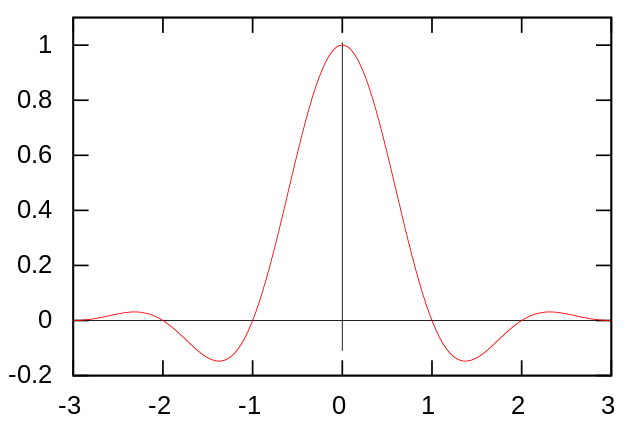
\includegraphics[width=0.9\columnwidth]{img/Lanczos-kernel.png}}{Lanczos Kernel}{fig:lanczos}

This means that if we want the windowing of the signal to not affect
its value, we need to window the data in the time domain with a sinc
function. Unfortunately, the sinc function has infinite support, which
implies that we would need to know all of the values of the entire
image to find the value of a single pixel. Lanczos Interpolation
involves using a windowed sinc function to give the function finite support:

\begin{equation}
  L(x) = \begin{cases}
    \mathrm{sinc}(x) \mathrm{sinc}(x/a) & \mathrm{if} -a < x < a\\
    0 & \mathrm{otherwise}\\
    \end{cases}
\end{equation}

Where $sinc$ is the function $\frac{\sin x}{x}$, and $a$ is a
parameter that determines the width of the window function. For the
purposes of this paper, an window size of 3 was chosen, as seen in
figure \ref{fig:lanczos}. 

\section{Drizzle Algorithm}

The bulk of the project was spent implementing the Drizzle
algorithm. Drizzle, also known as Variable Pixel Linear
Reconstruction, was developed while processing images from the hubble
space telescope. The basic premise of the drizzle algorithm, is there
exists a spectrum between interlacing the individual source pixels of
the image directly, and perfectly weighting the output pixels by the
amount of overlap. Figure \ref{fig:drizzle} shows the warping process
of the drizzle algorithm. First, the output pixel size is
determined. If we want to upscale the image, we can represent it here
by shrinking the virtual size of each output pixel.

\centerimage{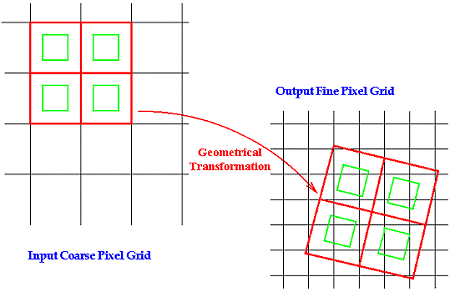
\includegraphics[width=0.9\columnwidth]{img/drizzle3.png}}{The
  Drizzle Algorithm}{fig:drizzle}

Intuitively, this means that each input pixel would overlap more than
one output pixel. The trick with the drizzling algorithm is to also
shrink the size of the input pixel as well. If we think of the input
pixel as being infinitely small, this corresponds to pure
interpolatoin: when warped to the destination pixels, each input pixel
only affects one output pixel. This results in the sharpest picture,
but if there is not enough input data to reconstruct the image, the
will be missing information for pixels in the output image.

The steps of the drizzling algorithm include:

\begin{enumerate}
\item draw a rectangle around each input pixel, and shrink by a factor
  of \textit{pixfrac}
\item Transform pixel rectangle using homography matrix
\item For each pixel in the neighborhood of the transformed quadrilateral:

  \begin{itemize}
    \item Calculate intersection of pixel and quadrilateral using
      Sutherland-Hodgman\cite{Sutherland:1974:RPC:360767.360802}
      algorithm.

    \item Calculate Area of intersection using Shoelace
      Formula\cite{meister1769generalia}

      \item Weight pixels based on area. 
  \end{itemize}
\end{enumerate}

While there are several open source implementations of the drizzle
algorithm available online, none of the ones I found were very
suitable. The IRAF\cite{tody1993iraf} astronomy package has an
implementation, however, it is written in fortran, and hard to port to
use with the OpenCV system.

There is another implementation in the STCSI\cite{betadrizzle}
scientific computing project. This implementation used some hard to
follow logic to determine the intersection of the warped pixels, and
so I undertook to write my own implementation in C.

\section{Results}
During the last full moon, I was able to go out and record some
video. A 2 minute video ended up containing over 2000 frames that were
used to evaluate the drizzle algorithm. The mean sharpness of the
output frame was calculated for the lanczos3 sharpening filter, as
well as the drizzle algorithm at two different \textit{pixfrac}
values, with various percentages of the images chosen, this can be seen in figure \ref{fig:sharpness}. 

\centerimage{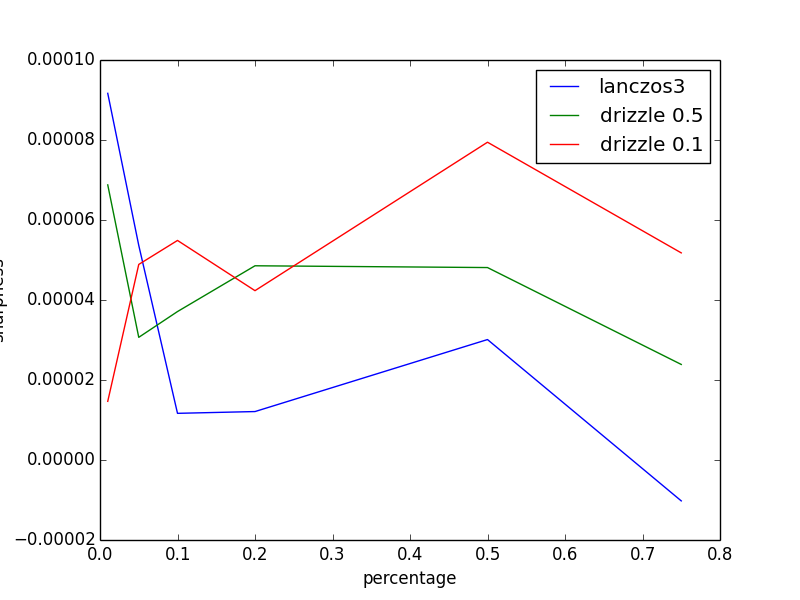
\includegraphics[width=0.9\columnwidth]{img/figure_1.png}}{Sharpness Results}{fig:sharpness}

The laplacian is not a perfect measure of sharpness: The issues at low
\textit{pixfrac} of missing pixels, is not captured in this
metric. However, it can plainly be seen that the overall sharpness of
the images tends to decrease as a larger percentage of the input
images are included in the final image.

\centerimage{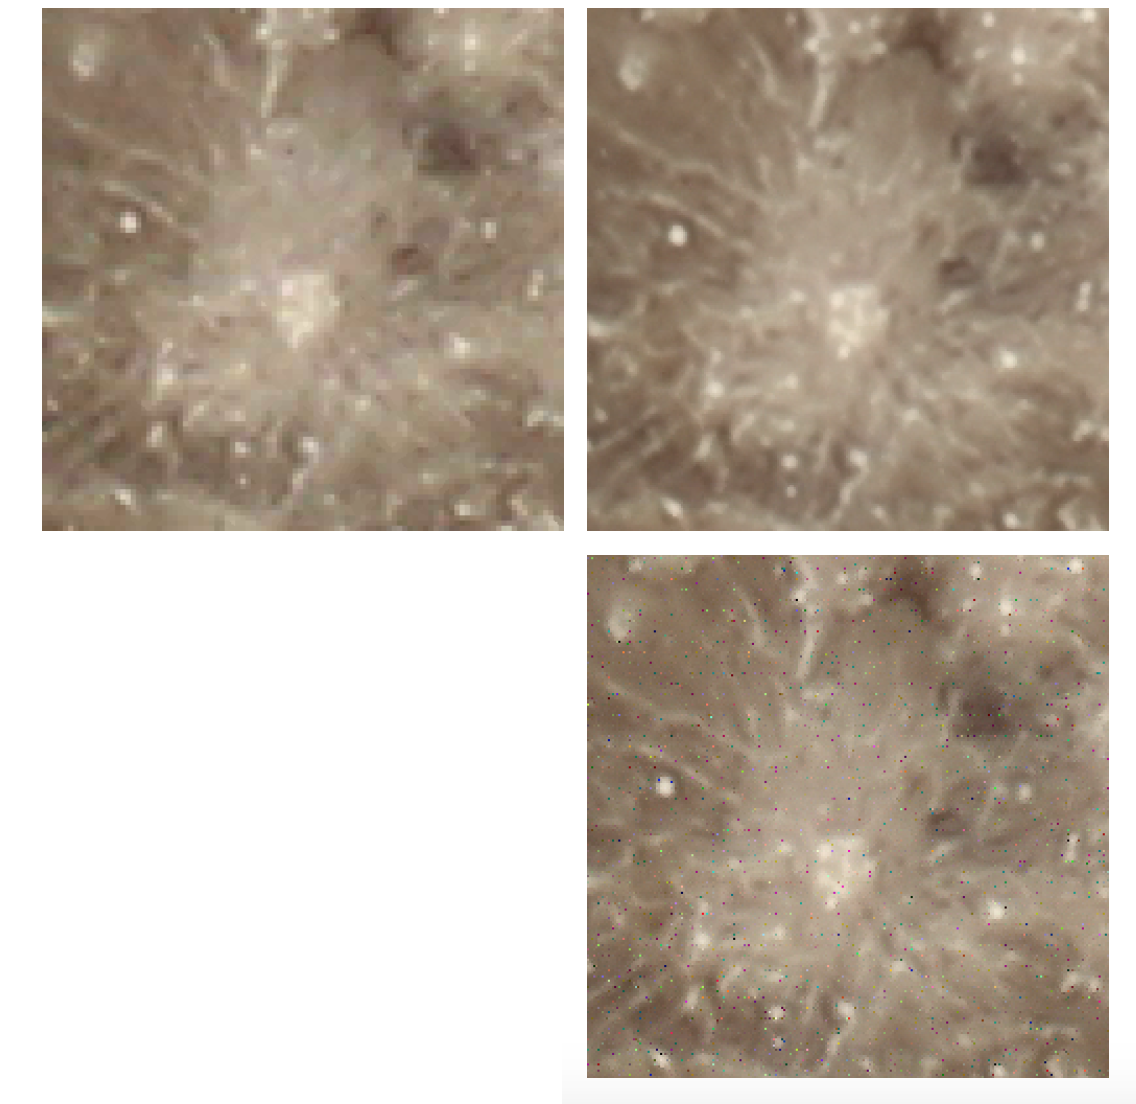
\includegraphics[width=0.9\columnwidth]{img/results1.png}}{Clockwise from top left: Source frame, drizzled, pixfrac=0.5, lanczos3 interpolation}{fig:results1}

Figure \ref{fig:results1} shows the results taken when the top 1\% of
images were integrated together. As you can see, the lanczos3
sharpening filter did not have enough information to fully fill in all
of the pixels of the output image. However, both the drizzled and
lanczos3 images show more detail than just a single raw image do.

\section{Conclusion}
Both the lanczos3 filtering method and the drizzling method increased
the effective resolution and sharpness of the output images. However,
I am not sure that the drizzle algorithm represents much of an
increase in quality versus just using lanczos interpolation. In
addition, more work needs to be done to develop an object way to
evaluate the sharpness of the images.

% bibliography goes here
\bibliographystyle{IEEEtran} \bibliography{IEEEabrv,citations}

\end{document}


